\documentclass{article}
\usepackage{graphicx}
\usepackage{amsmath}
\usepackage{esint}
\usepackage{subcaption}
\begin{document}
	
	\title{Introduction to Circuitry}
	\author{}
	
	\maketitle
	
	\begin{abstract}
	Transformers are one of the main devices in electric machinery alongside \textit{generators} and \textit{motors}.
	In this article we see how they work and why are they crucial in power transmission.
	\end{abstract}
	
	\section{Transformers: The Basics}
	Transformer is a device that takes an AC signal and produces an AC output with the same frequency, but a \textit{different voltage level}.
	Working principal of a transformer is \textit{Faraday's law of induction}:

	$$ \varepsilon = - \frac{d \phi}{dt} $$

	This physical law states that the induced \textit{electromotive force} (on a wire) is equal to the instantaneous rate of magnetic flux passing through it over time.\footnote[1]{A note here, the negative sign ($-$) merely implies that the induced voltage is in the opposite direction which the changed in flux happened; Hence it has no effect on the magnitude of induced voltage.}
	\textit{Flux} in general, is a measurement of how much a quantity is passing through a surface (magnetic field strength in this case).
	Hence it is defined as:
	
	$$ \phi = \iint\limits_S B.ds$$
	
	Where $B$ is the magnetic flux density (in units of \textbf{Tesla} or \textit{T} for short) \textit{dot-product}ed with differential surface elements $ds$ (in meters squared).
	Although this formula can be used to calculate any magnetic flux, in transformers we exclusively deal with fluxes that have (ideally) constant magnetic flux density.
	Therefore in this case we can simply use this formula instead:
	
	$$ \phi = B.A = BA\cos \theta$$
	
	($B$ magnetic flux density and $A$ area of surface.)
	
	Scientists dedicated a new unit for the flux which is called \textbf{Weber} or \textit{Wb}.
	Hence flux of 1 Weber is equivalent of a 1 meter surface passing 1 Tesla magnetic fields \textit{perpendicular} at each point of a surface.
	
	
	With our definition of magnetic flux for constant $B$ fields, we can write the \textit{law of induction} as:

	$$ \varepsilon = -\frac{d(B.A)}{d t} $$
	
	In electric machinery, the instantaneous change in magnetic flux typically happens in one of two cases.
	Either the magnetic field density is constant and the surface is changing (More accurately, the intersection between these constant magnetic density with a surface are rotationally changing); As it happens in \textit{generators}.
	Where the other case is when the surface is constant but the magnetic field density is changing; As we'll see this happens in the \textit{transformers}.

	There are number of ways to have a constant surface but \textit{changing} magnetic field.
	The most trivial one perhaps is to hold a permanent magnet near a conductor and rapidly sliding alongside it.
	This is a method that can be demonstrated in labs but it's not a useful case for us. 
	What we are interested instead, is the change in a changing magnetic field produces by a current-carrying wire. 
	In general, a current-carrying wire produces an magnetic field around it.
	The strength of this field can be obtained by:

	$$ B = \frac{\mu_o I}{2 \pi r} $$
	
	$I$ as current in unit of Amperes, $r$ as the distance from wire and $\mu_o$ a constant that makes the units work in the SI system.

	\begin{figure}[h!]
	\centering
	\begin{subfigure}[b]{0.8\linewidth}
		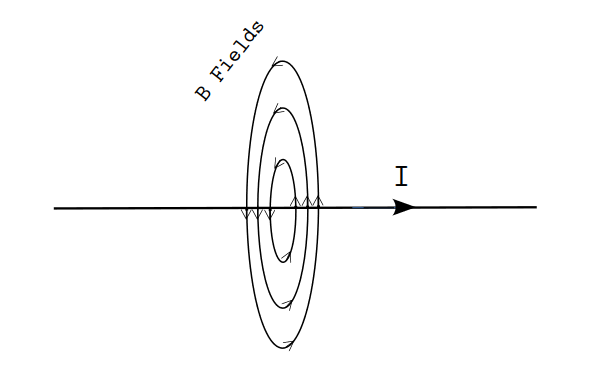
\includegraphics[width=\linewidth]{magnetic_field_around_a_wire.png}
	\end{subfigure}
	\end{figure}

	If we make a solenoid out of this wire, it forms a (nearly) uniform magnetic field strength inside of it \footnote[1]{We skip the proof here but it has a straightforward proof that can be found on the web.}:
	
	\begin{figure}[h!]
	\centering
	\begin{subfigure}[b]{0.7\linewidth}
	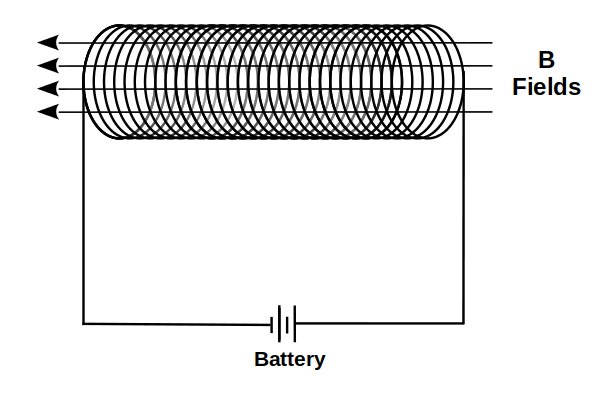
\includegraphics[width=\linewidth]{solenoid.png}
	\end{subfigure}
	\end{figure}
	
	In this case, the strength of this magnetic field can be calculated by:
	
	$$ B = \mu_o N I / L$$
	
	($N$ is number of wire turns and $L$ the (?) length of the solenoid.)
		
	When we have an solenoid and a current starts passing through it, by law of induction, voltage gets induced in the solenoid (in the same wires that was making it up).
	This voltage is also called \textbf{back EMF} and is always opposing the change in current.\footnote[1]{The component \textit{inductor} we saw in Article 1 was exactly a type of solenoid; With the difference that inductors also of a core. Presence of a core makes their induction effect stronger.}
	Note that an ideal solenoid that has no resistivity doesn't consume nor generates any electrical power; But merely holds it.
	For example, if a \textit{back EMF} was caused as an effect of instantaneous positive change in the current, same voltage would apply when it wanted to drop i.e. having a negative instantaneous change in the current later on.
	
	If we have a tightly wound solenoid, we can write the formula of induction as:
	
	$$ \varepsilon = -N\frac{d\phi}{dt} $$
	
	($N$ is the number of wire turns and $\phi$ the flux produced by \textit{each} loop)
	
	\subsubsection{Solenoid connected to an AC Source}	
	When the electrical source of a solenoid is sinusoidal AC signal, the flux getting produced inside of it gets a sinusoidal form as well:
	
	$$ \phi(t) = \phi_{m} \sin \omega t $$
	
	Substituting into the formula of induction:
	
	$$ \varepsilon = -N \frac{d\phi}{dt} = - N \frac{d (\phi_{m} \sin \omega t)}{dt} = -N \frac{\phi_{m} d (\sin \omega t)}{dt} = N \phi_{m} \omega \cos \omega t $$
	
	Which implies that having a sinusoidal flux makes the induced voltage on the solenoid sinusoidal as well.
	Calculating \textit{RMS} for this function we get:
	
	$$ \varepsilon_{rms} = \frac{N \phi_{m} \omega}{\sqrt{2}}$$
	
	And since the coils in a solenoid have a constant surface, this formula can also be written as:
	
	$$ \varepsilon_{rms} = \frac{N B_{m} A (2\pi f)}{\sqrt{2}} \approx 4.44NB_{m}Af $$
	
	($N$ is number of turns, $B_m$ Maximum field density, $A$ surface and $f$ frequency)
		
	\subsection{Transformers: Basic Construction}
	
	What happens if we hold two solenoids close to each other in a way that the magnetic flux of one solenoid passes through the other one as well? (ideally all of it).
	
	\begin{figure}[h!]
	\centering
	\begin{subfigure}[b]{0.9\linewidth}
		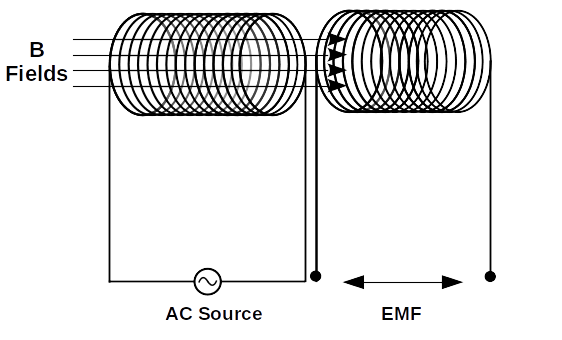
\includegraphics[width=\linewidth]{basic_transformer.png}
	\end{subfigure}
	\end{figure}
	
	
	In this setup if we connect a sinusoidal AC source to one of these coils, not only an \textit{EMF} gets induced in the first coil, but also in the second coil as well.
	This effect comes from the fact that the magnetic flux of the first coil (hence its change over time) passes through the second one too. 
	Let's denote the first one $E_1$ and the latter as $E_2$.
	These values can be obtained by:
	
	\begin{align*}
	& E_1 = 4.44N_1B_{m}Af \\
	& E_2 = 4.44N_2B_{m}Af
	\end{align*}
	
	And since all of these parameters except $N_1$ and $N_2$ are same for both of these coils, we can simply divide them to get their ratio:
	
	\begin{equation}
	\frac{E_1}{E_2} = \frac{N_1}{N_2}
	\end{equation}
	
	This relation simply means that the ratio of induced voltage on each side is proportional to the number coil turns in that side.
	The setup we have here is the basic construction of a transformer and equation (1) is the main formula we use to describe a transformer.
	For short it is also written as \textit{$N_1$:$N_2$}.
	For example a \textit{1:10} transformer increases the voltage level of a sinusoidal AC signal by the multiple of $10$.
	
	The ratio $\frac{N_1}{N_2}$ of a transformer is also called \textit{turn ratio} and is denoted by \textbf{a}:
	
	$$ \frac{N_1}{N_2} = a $$
	
	An ideal transformer doesn't consume nor generate any power\footnote[1]{The reason for this property comes from physical properties of transformers.
	Specifically the effect of 'Special Relativity'.
	Although understanding this theory doesn't directly affect how we understand the working of these devices, we would still have a look at this theory in a separated article and how does the 'magnetic effect' gets created in the first place.};
	Hence the input and output power remain the same.
	This means that the change in voltage level of output is accompanied by change in its current level, by amount that the formula of power $P(t) = V(t).I(t)$ gives the same value for the output as input. 
	
	$$ P_1 = P_2$$
	$$ E_1.I_1 = E_2.I_2$$

	Therefore:
	
	$$ \frac{E_1}{E_2} = \frac{I_2}{I_1} = a $$
	
	(all functions of time $t$)	
	
	One thing to note that is in real transformers, the wire turns are wrapped around a ferromagnetic material such as iron.
	The presence of this core makes the induction effect stronger.
	
	\subsubsection{Impedance transfer in Transformers}
	When we have a transformer with load on the secondary side:
		
	\begin{figure}[h!]
	\centering
	\begin{subfigure}[b]{0.45\linewidth}
		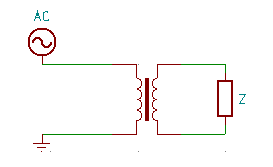
\includegraphics[width=\linewidth]{with_impedance.png}
	\end{subfigure}
	\end{figure}
	
	Using transformer formula we can calculate how does this load is seen from the primary side's perspective.
	For an ideal transformer:

	$$ E_1.I_1 = E_2.I_2$$
	
	From Ohm's law:
	
	$$E = ZI$$
	
	Therefore:
	
	$$ Z_1.I_1^2 = Z_2.I_2^2$$
	$$ \frac{Z_1}{Z_2} = (\frac{I_2}{I_1})^2 = a^2$$	
	$$ Z_1 = Z_2a^2$$
	
	With this formula we can replace the transformer and it's secondary side load, by a single load $Z_1$. This process is called \textit{impedance transfer}.
	
	\subsection{Equivalent circuit of a real Transformer}
	In practice, a real transformer doesn't produce the same power for output as input.
	This difference is caused by voltage drop in the resistivity of coils, the core and other factors we will discuss in this section.
	Let's first see what is the equivalent circuit of a real transformer, then we would ration about it's each part.
	
	\begin{figure}[h!]
	\centering
	\begin{subfigure}[b]{1\linewidth}
		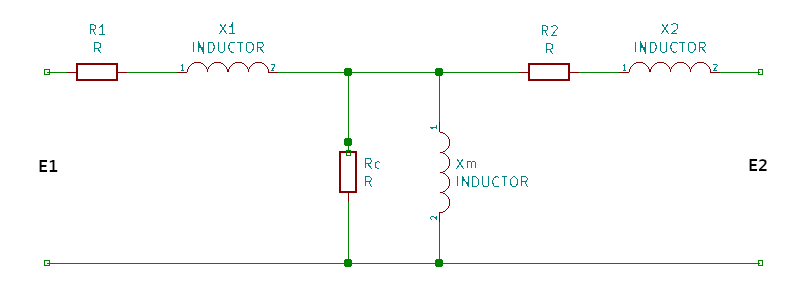
\includegraphics[width=\linewidth]{real_transformer.png}
	\end{subfigure}
	\end{figure}
	
	As shown in the diagram, this circuit is made up by both \textit{series} and \textit{parallel} elements.
	
	The series elements are the result of the \textit{coils} in each side. More precisely, $R_1$ and $R_2$ are due resistivity and the inductor elements $X_1$ and $X_2$ due the main inductive effect of the coils respectively.
	
	The parallel elements $R_c$ and $X_m$ are core losses of the transformer.
	$R_c$ is called \textit{magnetization resistivity} and $X_m$ is the effect of \textit{flux leakage}.
	Flux leakage is the flux that doesn't get fully captured by the other side (in some sense it gets "wasted").
	We can think of this leakage, analogous by having a simple inductor without it's flux getting passed to the other one. Notice that these two elements are in parallel to each other because the effect these impedances affect independently yet simultaneous with each other.
	
	This complicated equivalent circuit can be simplified for power transformers with few approximations.
	In transformers the current that flows through the parallel elements ($R_c$ and $X_m$) is a fraction of the current in series elements.
	With this physical property we can remove the parallel elements in practical sense, thus simplifying the equivalent circuit greatly to:
		
	\begin{figure}[h!]
	\centering
	\begin{subfigure}[b]{0.8\linewidth}
		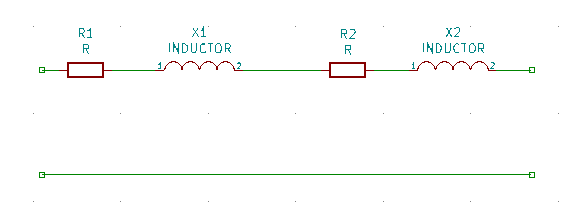
\includegraphics[width=\linewidth]{transformer_approx1.png}
	\end{subfigure}
	\end{figure}
	
	Therefore by substituting with equivalent elements:
	
	\begin{figure}[h!]
	\centering
	\begin{subfigure}[b]{0.6\linewidth}
		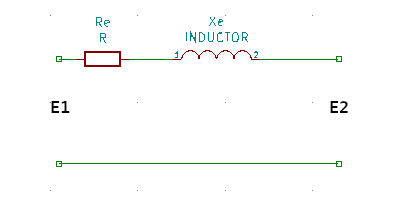
\includegraphics[width=\linewidth]{transformer_approx2.png}
	\end{subfigure}
	\end{figure}
	
	Furthermore if the transformer is designed for more than 1 MVA powers, the impedance of resistance element $R_e$ is negligible compared to the inductance $X_e$ therefore can be discarded. 
	Hence:
	
	\begin{figure}[h!]
	\centering
	\begin{subfigure}[b]{0.5\linewidth}
		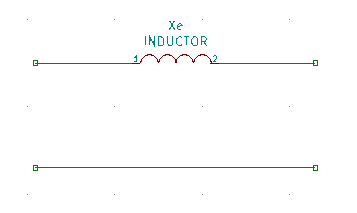
\includegraphics[width=\linewidth]{transformer_approx3.png}
	\end{subfigure}
	\end{figure}
	
	This circuit is as simplified as we can get and it's used for modeling power transformers in engineering applications.
	
	\subsection{Measuring the values of the equivalent circuit}
	So far we've seen the equivalent circuit for a real transformer. 
	But how can we find the values of it's components? In this regard we perform two physical experiments on our transform namely \textit{open-circuit} and \textit{short-circuit} test. 
	With these tests, the parameters of equivalent circuit can be measured with a very good approximation.
	
	\subsubsection{open-circuit test}
	With this experiment we can find the values of parallel elements: $X_m$ and $R_c$. The way that this test works is as follows:

	1. We open-circuit one side of the transformer.
	
	2. While the side is open-circuited, we apply the maximum line voltage to the other side and simultaneously we measure power and current on the side as well.

	Since there is no load on the secondary side, a current will flow through the first series element ($R_1$ and $X_1$) as well as the excitation branch ($R_c$ and $X_m$). 
	The impedance of series elements are substantially lower than the elements in excitation branch.
	Hence we can conclude that approximately all the voltage drop of our input signal has occurred in the excitation branch.
		
	Now that we have the value of input voltage (from our source) and we measured the power and current as well, we can use these formulas to calculate the elements $R_c$ and $X_m$.
	
	$$ \cos \phi = \frac{P}{U I} $$
	$$ \sin \phi = \sqrt{1 - \cos^2 \phi}$$
	$$I_c = I \cos \phi $$
	$$I_m = I \sin \phi $$
	$$X_m = \frac{U}{I_m} $$
	$$R_c = \frac{U}{I_c}$$
	
	($P$ and $I$ are the measured power and current respectively, and $U$ the applied voltage from our source.)
	
	A note here: In step (2) we choose the low-voltage side for measurements because it's safer and easier to work with.
	\subsubsection{short-circuit test}
	This experiment is performed to determine the values of series elements. 
	The steps are:

	1. We short-circuit one side of the transformer.

	2. While the side is short-circuited, we slowly increase the voltage on the other side until we get the maximum line \textit{current}; And as before, we measure both power and current as well.

	Since the secondary side is short-circuited, applying a very small voltage in the primary side causes maximum current to flow in the transformer.
	Small voltage different between two input terminals means that the current that flows in the parallel elements ($R_c$ and $X_m$) is negligible and therefore can be ignored.
	This approximation implies that all voltage drop in this experiment is caused by the series elements.
	
	Having the measurement values:
	
	$$ P = (R_1 + R_2)I^2 $$
	$$ P = R_e I^2 $$
	$$ R_e = \frac{P}{I^2} $$
	$$ Z_e = \frac{U}{I} $$
	$$ X_e = \sqrt{Z_e^2 - R_e^2}$$

	(As before $P$ and $I$ are the measured power and current respectively, and $U$ the applied voltage from our source.)
	
	
	\subsection{Applications of Transformers}
	Transformers are used in circuits that need a change in voltage/current level such as audio amplifiers in electronic devices.
	But the most trivial and arguably crucial application of transformers are in power transmission. 
	
	We often need to transmit electrical power energy over large distances, due the fact that generators are often apart from the consumers (factories, urban users, etc). These wires that transmit these electrical powers from generators to consumers have some resistivity just like any other wire, and from Ohm's law the voltage drop across these wires are calculated by:
	
	$$V = RI$$
	
	By knowing the voltage drop, to calculate the power consumption in these wires (which is getting wasted and getting converted to heat) we need to multiply it by its current $I$:
	
	$$P_{wires} = RI^2 $$
	
	Which tells us is that the power loss in the lines are proportional to the square of its current $I$.
	This is where transformers come in use.
	These devices decrease the current (while keeping the same power by increasing voltage level); Hence decreasing the power loss in these wire substantially.
	These kind of transformers are also known as \textit{step up transformers}.
	
	Since the end point of the power lines receive huge voltages, we need to use transformers again but this time to decrease the voltage (hence increasing the current).
	We do this process to make the voltage level in a safe and usable level. These transformers that decrease the voltage level are also known as \textit{step down transformers}.
	
	The types of transformers we discussed in this article are known as \textit{single-phase} transformers and they operate with power lines consisting of a single phase signals. 
	Although the most transformers that are used in practice are \textit{three-phase}, the basic concepts behind them are similar to single-phase ones.
	
	These documents are published under an open license (see the project's root directory for more info), and were intended to be part of an open and a collaborative project. Feel free to fork this document, send pull request and also give your feedback. Thanks for reading!
	
\end{document}
